\documentclass[a4paper, 12pt]{article}
\usepackage{geometry}
\geometry{margin=2cm}
\usepackage{graphicx} % Required for the inclusion of images
\usepackage[utf8]{inputenc}
%\usepackage{natbib} % Required to change bibliography style to APA
\usepackage{amsmath} % Required for some math elements 
\usepackage[spanish]{babel} 
%\usepackage{fontspec}
\usepackage{lineno,hyperref}
\usepackage{upgreek}
\usepackage{gensymb}
\usepackage{textcomp}
\usepackage{amssymb}
\usepackage{textgreek}
\usepackage{float}
\usepackage{fancyhdr}
\usepackage{dirtytalk}

\allowdisplaybreaks
%\textwidth18cm
%\textheight22cm
%\topmargin0cm
%\oddsidemargin2cm
%\hypersetup{hidelinks}

\usepackage{multirow}

\hypersetup{
    colorlinks=true,
    linkcolor=blue,
    }
\graphicspath{{img}}
\setlength\parindent{0pt} % Removes all indentation from paragraphs

\renewcommand{\labelenumi}{\alph{enumi}.} % Make numbering in the enumerate environment by letter rather than number (e.g. section 6)

\renewcommand{\b}{\textbf}

\newsavebox{\mygraphic}
\sbox{\mygraphic}{
\includegraphics[height=1cm]{logoUNRN.jpg}}


\pagestyle{fancy}

\fancyhead{}

\headheight 16pt

\fancyhead[LO]{\setlength{\unitlength}{1in}
	\begin{picture}(0,0)
		\put(0,0){\usebox{\mygraphic}}
	\end{picture}
	\hspace{1cm}
}

\fancyhead[CO] {\hspace{1.5cm} \large Física I: Ingenierías Ambiental, Electrónica y Telecomunicaciones}

%esto me pareció piola para enumerar los ejercicios
%lo saqué de acá: https://tex.stackexchange.com/questions/302948/numbered-exercises-as-sections
%%%%%%%%%%%%%%%%%%%%%%%%%%%%%%%%%%%%%%%%%5
\newcounter{eje}
\setcounter{eje}{0}
\newcounter{subeje}
\setcounter{subeje}{-1}
\renewcommand\thesubeje{\arabic{eje}\alph{subeje}}%
\newcommand \eje{%
  \vspace{.2cm}
  \par\noindent
  \ifnum\value{subeje}>-1
    \refstepcounter{subeje}%
    \llap{\thesubeje)\quad}%
  \else
    \refstepcounter{eje}%
    \llap{\theeje)\quad}%
  \fi
}
\begin{document}
\pagestyle{fancy}

\begin{center}

	{\Large \textbf{Final Física I (Septiembre)}}
 
\vspace{.2cm}

{jueves 7/9}
\end{center}

Tome para el valor de g = 9.8 m/s$^2$.

\eje Un aro de basquet está colocado a una altura h$_1$ = 3.05 m del suelo y el centro del aro se encuentra a una distancia horizontal L = 5.425 m del lugar donde se efectúan los libres. Un jugador está efectuando tiros libres desde esa distancia. Si la pelota abandona su mano cuando se encuentra exactamente a la distancia de libres y a una altura h$_2$ = 2.45 m del piso con un ángulo $\alpha$= 48$\degree$ respecto del suelo (ver figura adjunta): 

a) Calcule algebraicamente la velocidad inicial v$_0$ en función exclusivamente de g, L, h$_1$ y h$_2$ y $\alpha$.

b) Evalúe con los datos del problema y calcule el valor para la velocidad inicial. 

\begin{figure}[H]
\begin{center}
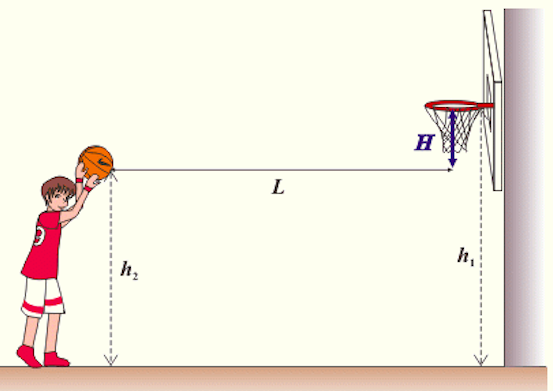
\includegraphics[clip,width = .45\columnwidth]{img/figura-final-septiembre-0.png}
\end{center}
\end{figure}

\eje Un satélite de masa 300 kg está en órbita circular alrededor de la Tierra a una altitud igual a la del radio medio de nuestro planeta (ver la figura adjunta). 

a) Encuentre (haciendo uso de R = $6.37\times 10^6$ m y M$_{Tierra}$ = $5.98\times 10^{24}$ kg) la velocidad orbital del satélite.

\begin{figure}[H]
\begin{center}
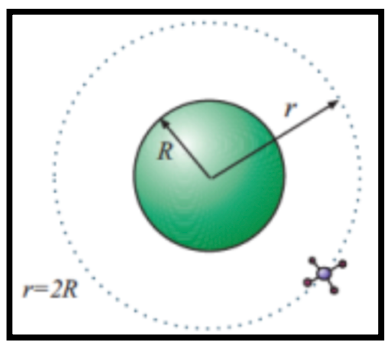
\includegraphics[clip,width = .45\columnwidth]{img/figura-final-septiembre-1.png}
\end{center}
\end{figure}

\eje Una joven tira de un trineo cargado de masa m = 20 kg sobre una superficie horizontal cubierta de nieve (ver figura adjunta). Considere que la velocidad del trineo es constante. Por otro lado, tome el coeficiente de fricción cinética $\mu_k$ entre el trineo y el suelo de 0.1, y el ángulo $\phi$ entre la soga y el suelo de 30$\degree$. Encuentre:

a) La aceleración del trineo. 

b) La magnitud de la tensión, de la fuerza normal y de la fricción sobre el trineo. 

\begin{figure}[H]
\begin{center}
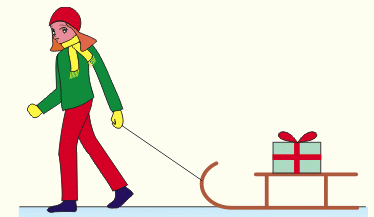
\includegraphics[clip,width = .45\columnwidth]{img/figura-final-septiembre-2.png}
\end{center}
\end{figure}

\eje Un disco de masa 10 kg y diámetro 1 m, y grosor despreciable rueda sin deslizar por un plano inclinado, el que forma un ángulo de 30$\degree$ con la horizontal del suelo. Encuentre la velocidad del centro del disco luego de recorrer una distancia de 5 m por el plano, suponiendo que el mismo parte del resposo. Ignore la pérdida de energía por rozamiento entre el disco y el plano inclinado, y recuerde que el momento de inercia de un disco de estas características, tomando el eje que pasa por su centro es de I = mR$^2$ con R el radio del disco. 

\eje \textbf{[PRÁCTICA 8, EJERCICIO 8]} En el dispositivo de la figura, una masa m es colgada de una cuerda que pasa sobre una
polea. El otro extremo de una cuerda es conectada a un generador de frecuenci 'f' fija. La cuerda
tiene una longitud 'l' = 2 m y una densidad lineal de 0.002 kg/m. Se observan armónicos
únicamente cuando las masas colgadas son de 16 y 25 kg, respectivamente.

a) ¿Cuáles son los armónicos producidos por estas masas?

b) ¿Cuál es la relación entre las tensiones y el número armónico?

c) ¿Cuál es la frecuencia del generador?

d) ¿Cuál es el valor máximo de 'm' para que se produzca un armónico?

\begin{figure}[H]
\begin{center}
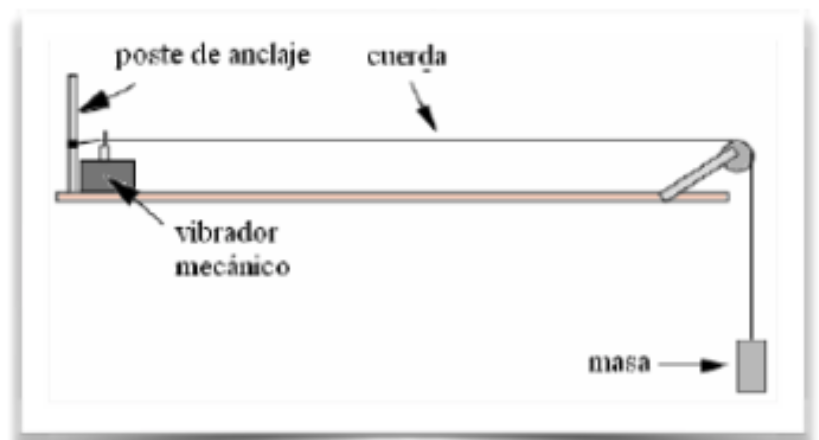
\includegraphics[clip,width = .45\columnwidth]{img/figura-final-septiembre-3.png}
\end{center}
\end{figure}

\eje \textbf{[PRÁCTICA 9, EJERCICIO 3]} Una pelota de plástico tiene 25 cm de radio y flota en agua con el 25\% de su volumen sumergido:

a) ¿qué fuerza deberemos aplicar a la pelota para sostenerla en reposo totalmente sumergida en
agua?

b) Si se suelta la pelota, ¿qué aceleración tendrá en el instante en que se suelte?

\end{document}